\documentclass{article}

% if you need to pass options to natbib, use, e.g.:
%     \PassOptionsToPackage{numbers, compress}{natbib}
% before loading neurips_2019

% ready for submission
% \usepackage{neurips_2019}

% to compile a preprint version, e.g., for submission to arXiv, add add the
% [preprint] option:
%     \usepackage[preprint]{neurips_2019}

\usepackage[final]{neurips_2019}
% to compile a camera-ready version, add the [final] option, e.g.:
% to avoid loading the natbib package, add option nonatbib:
%     \usepackage[nonatbib]{neurips_2019}
\usepackage{multirow}
\usepackage[utf8]{inputenc}
\usepackage[T1]{fontenc}
\usepackage{hyperref} 
\usepackage{url} 
\usepackage{booktabs}
\usepackage{amsfonts} 
\usepackage{nicefrac} 
\usepackage{microtype}  
\usepackage{graphicx}
\usepackage{float}
\usepackage{graphicx}
\usepackage{adjustbox}
\usepackage{subcaption}
\usepackage{amssymb}
\usepackage[namelimits]{amsmath} 
\newcommand{\ra}[1]{\renewcommand{\arraystretch}{#1}}


\title{

(Re-)Imag(in)ing Price Trends}

% The \author macro works with any number of authors. There are two commands
% used to separate the names and addresses of multiple authors: \And and \AND.
%
% Using \And between authors leaves it to LaTeX to determine where to break the
% lines. Using \AND forces a line break at that point. So, if LaTeX puts 3 of 4
% authors names on the first line, and the last on the second line, try using
% \AND instead of \And before the third author name.

\author{%
  Fu Yang(21029346) \\
  \texttt{yfubo@connect.ust.hk} \\
  \And
  Luo Yuqing(20582315)\\
  \texttt{yluobb@connect.ust.hk} \\
  \AND
  Wang Jinyuan(21028990)\\
  \texttt{jwangiy@connect.ust.hk} \\
  \And
  Wang Tong(20905737) \\
  \texttt{twangce@connect.hk} \\
}

\begin{document}

\maketitle

\begin{abstract}

In this report, we endeavor to replicate and expand upon the insightful findings presented in the publication titled "(Re-) Imag(in)ing Price Trends" [1]. The original work delves into the fascinating realm of utilizing convolutional neural networks (CNN) as a means to comprehend stock price patterns depicted in image form, ultimately enabling the prediction of future returns. Our replication efforts are centered around faithfully reproducing the data processing techniques, CNN model construction, and training methodologies outlined within the original study. Moreover, we have taken the opportunity to extend the research by embarking on several additional investigations, including ablation studies, visualized interpretation using Grad-CAM, and exploration of regression. To ensure a comprehensive and coherent presentation, this report is thoughtfully divided into six distinct sections: Introduction, Data, Architecture Design, Working Flow, Extension, and Conclusion. These sections collectively provide a comprehensive account of our replication efforts, extensions, and the insights gained from our study.


\end{abstract}

\section{Introduction}

Predicting future stock returns from historical price movements is a topic of great interest, but traditional empirical finance methods may struggle to provide accurate results due to the subtle and complex patterns embedded in stock prices. In this report, we approach the analysis of price trends from a machine learning perspective.

Given the features that significantly influence stock prices remain elusive, the convolutional neural network is an apt alternative since it possesses the flexibility to extract predictive signals from raw input data. To leverage the advantages of automated signal generation, we transform historical stock prices to images, which are typical input for CNN models, and train the panel CNN model to predict the future direction of stock returns. 

\section{Data}
\subsection{Data description}

In accordance with the article titled "(Re-) Imag(in)ing Price Trends", our empirical analysis revolves around a panel prediction model for US stock returns using data from 1993 to 2020. The input data for this model depicts price and volume information over different time periods. Specifically, the data represents daily open, close, high, and low prices, as well as daily trading volume and moving average prices over the past 5, 20, and 60 days in the original paper. Our report focuses solely on the 20-day moving average. This decision is based on the notion that the long horizon entails a more complex network structure, which may impede computational efficiency. Conversely, the short horizon might oversimplify the analysis, potentially compromising the robustness of the conclusions drawn. Figure 1 displays a portion of the original data that was utilized to assess the accuracy of our predictions in subsequent analyses.

\vspace{10pt}
\begin{figure}[H]
	\centering
	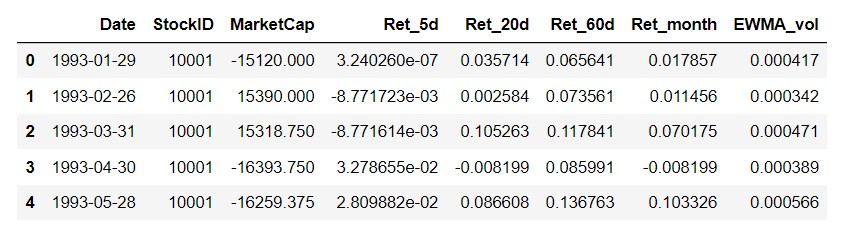
\includegraphics[width=0.8\textwidth]{1_2Examples of Original Data.jpg}
	\caption{Examples of Original Data}
\end{figure}

To facilitate analysis, the original dataset was partitioned into three distinct categories based on the returns observed. Within this categorization, a value of 0 was assigned to instances characterized by non-positive returns. Conversely, instances exhibiting positive returns were assigned a value of 1.

\subsection{Data processing}
The data processing stage involves further transformations and modifications to the prepared dataset. 

The primary objective of transforming the original one-dimensional time series of stock data into two-dimensional images is to improve the prediction accuracy of the model. The use of images in this approach offers advantages for stock price trend prediction. CNNs excel at image analysis, enabling effective feature extraction. Converting time series into images captures important relationships and trends visually. Combining price and trading volume data within images enhances the model's understanding. This image encoding approach is suitable for technical trading analysis, aiming to forecast stock price trends.

The original paper's images have unique characteristics, with daily data consolidated into 20-day intervals and standardized height for easy comparison. "OHLC" bars are used instead of candlestick charts, optimizing visual space. Additional features like moving averages and volume bars enhance representation. To optimize efficiency, image data is transformed into binary form, reducing memory requirements and enabling faster computations.

\begin{figure}[H]
	\centering
	\begin{minipage}[b]{0.4\linewidth}
		\centering
		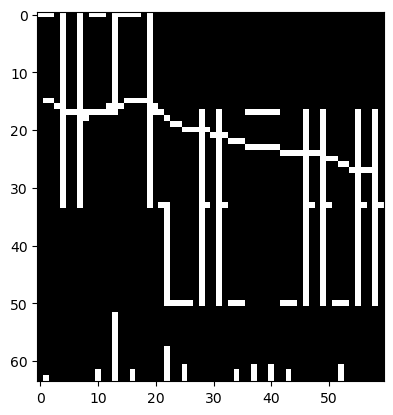
\includegraphics[width=0.6\linewidth]{2_1Examples of Final Image.png} 
	\end{minipage}
	\hfill
	\begin{minipage}[b]{0.4\linewidth}
		\centering
		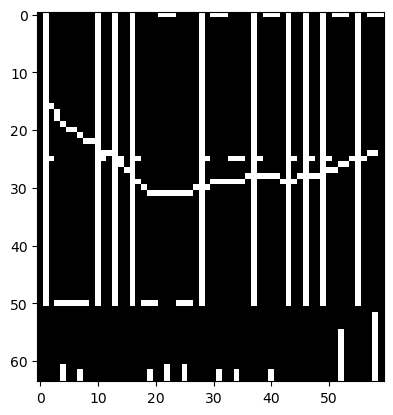
\includegraphics[width=0.6\linewidth]{2_2Examples of Final Image.png} 
	\end{minipage}
	\caption{Examples of Final Image}
\end{figure}

After extensive efforts, we successfully generated an image(e.g. Figure 2)that incorporates the stock price, moving average lines, and volume bars. These features were carefully designed to be compatible with the CNN model, ensuring optimal utilization of the image representation for analysis and prediction purposes.

\section{Architecture Design}
A Convolutional Neural Network (CNN) is a deep learning algorithm designed for image analysis and object recognition. It takes an input image, identifies important objects within it, and distinguishes one object from another. By stacking together a sequence of operations, a CNN transforms a raw image into a set of predictive features and makes a final prediction.  

The key operations in a CNN's building block are convolution, activation, and pooling.

\subsection{Convolution}
Convolution is a process that is similar to kernel smoothing. It involves scanning an image both horizontally and vertically. For each element in the image matrix, a summary of the surrounding area is computed.

In convolution, a set of filters is used. A filter is a small matrix of weights.In our project, 64 filters were employed, each with a kernel size of 5x3. We use 3 blocks for 20-day images. 

To safeguard the data from loss, a padding function is added. Padding involves adding extra pixels to each side of the image to prevent the feature map from becoming too small. The number of pixels added is determined by the size of the filter and the stride. 

So here we applies a 2D convolution over an input signal composed of several input planes with ‘CONV2D’,
\begin{itemize}
    \setlength\itemindent{2em}
    \item[$\bullet$] \emph{Input: $(N, C^{in}, H^{in}, W^{in})$ or $(C^{in}, H^{in}, W^{in})$}

    \item[$\bullet$] \emph{Output: $(N,C^{out}, H^{out}, W^{out})$ or $(C^{out}, H^{out}, W^{out})$}, where \\
    
    \emph{$H^{out} = \left\lfloor\frac{H^{in} + 2 * padding[0] - dilation[0] * (kernel\_size[0]-1)-1}{stride[0]} + 1 \right\rfloor$}
    
    \emph{$W^{out} = \left\lfloor\frac{W^{in} + 2 * padding[1] - dilation[1] * (kernel\_size[1]-1)-1}{stride[1]} + 1\right\rfloor$}
    
\end{itemize}

For example, on the first layer the first operation is a Conv2d layer with an input of 1 channel, outputting 64 channels. It uses a kernel size of (5, 3), a stride of (3, 1), padding of (30, 1), and dilation of (2, 1).  

Furthermore, batch normalization is incorporated into the design of the CNN model to counteract overfitting. Here we applies Batch Normalization over a mini-batch of 2D inputs with additional channel dimension with ‘BATCHNORM2D’, and in the shape,

\begin{itemize}
    \setlength\itemindent{2em}
    \item[] $y = \frac{{x - E[x]}}{{\sqrt{{\text{{Var}}[x] + \epsilon}}}} \cdot \gamma + \beta$
    
    \item[$\bullet$] Input: \emph{(N, C, H, W)}
    
    \item[$\bullet$] Output: \emph{(N, C, H, W)} (same shape as input)
\end{itemize}
The second operation of batch normalization is a BatchNorm2d layer with 64 channels. 

\subsection{Activation}
In a Convolutional Neural Network, the activation operation is a crucial step that follows the convolutional operation. It introduces non-linearity into the network, enabling it to learn complex patterns and make accurate predictions. The activation operation applies a non-linear transformation element-wise to the output of a convolutional filter.

The choice of the activation function plays a significant role in the effectiveness of the CNN. In the case you mentioned, the "leaky ReLU" activation function is used. The leaky ReLU addresses the limitation of the standard ReLU activation function, known as the "dying ReLU" problem. 

\begin{figure}[H]
	\centering
 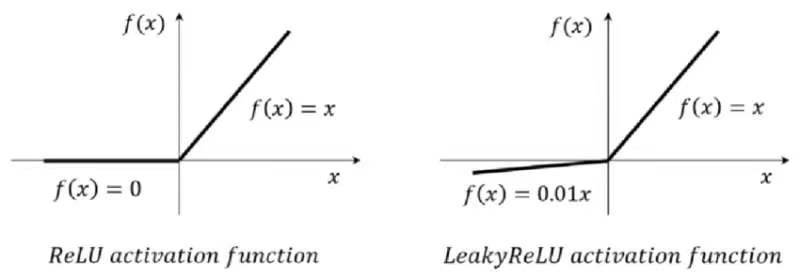
\includegraphics[width=0.5\linewidth]{2_3ReLU-activation-function-vs-LeakyReLU-activation-function.jpg}
	\caption{ReLU-activation-function-vs-LeakyReLU-activation-function}
\end{figure}

For example, On layer1 the second operation is a BatchNorm2d layer with 64 channels. And the third operation is a LeakyReLU activation function with a negative slope of 0.01.

\subsection{Pooling}

Pooling in a convolutional neural network reduces data dimensionality, removes redundancy, and enhances the network's robustness by focusing on important features while suppressing noise. It improves computational efficiency, memory usage, and generalization to new data.

Here we applies a 2D max pooling over an input signal composed of several input planes with ‘MAXPOOL2D’, and in this shape

\begin{itemize}
    \setlength\itemindent{2em}
    \item[$\bullet$] \emph{Input: $(N, C, H^{in}, W^{in})$ or $(C, H^{in}, W^{in})$}
    
    \item[$\bullet$] \emph{Output: $(N,C, H^{out}, W^{out})$ or $(C, H^{out}, W^{out})$}, where \\
    
    \emph{$H^{out} = \left\lfloor\frac{H^{in} + 2 \times \text{{padding}}[0] - \text{{dilation}}[0] \times (\text{{kernel\_size}}[0]-1)-1}{\text{{stride}}[0]} + 1 \right\rfloor$}
    
    \emph{$W^{out} = \left\lfloor\frac{W^{in} + 2 \times \text{{padding}}[1] - \text{{dilation}}[1] \times (\text{{kernel\_size}}[1]-1)-1}{\text{{stride}}[1]} + 1\right\rfloor$}
\end{itemize}

For example, On layer1 the fourth operation is a MaxPool2d layer with a kernel size of (2, 1), a stride of (3, 1), padding of (0,1), and dilation of (2, 1).

The final architecture of the baseline model is as the Figure 3 shows below.

\begin{figure}[H]
	\centering
	\begin{minipage}[c]{0.4\linewidth}
		\centering
		\adjustbox{valign=c}{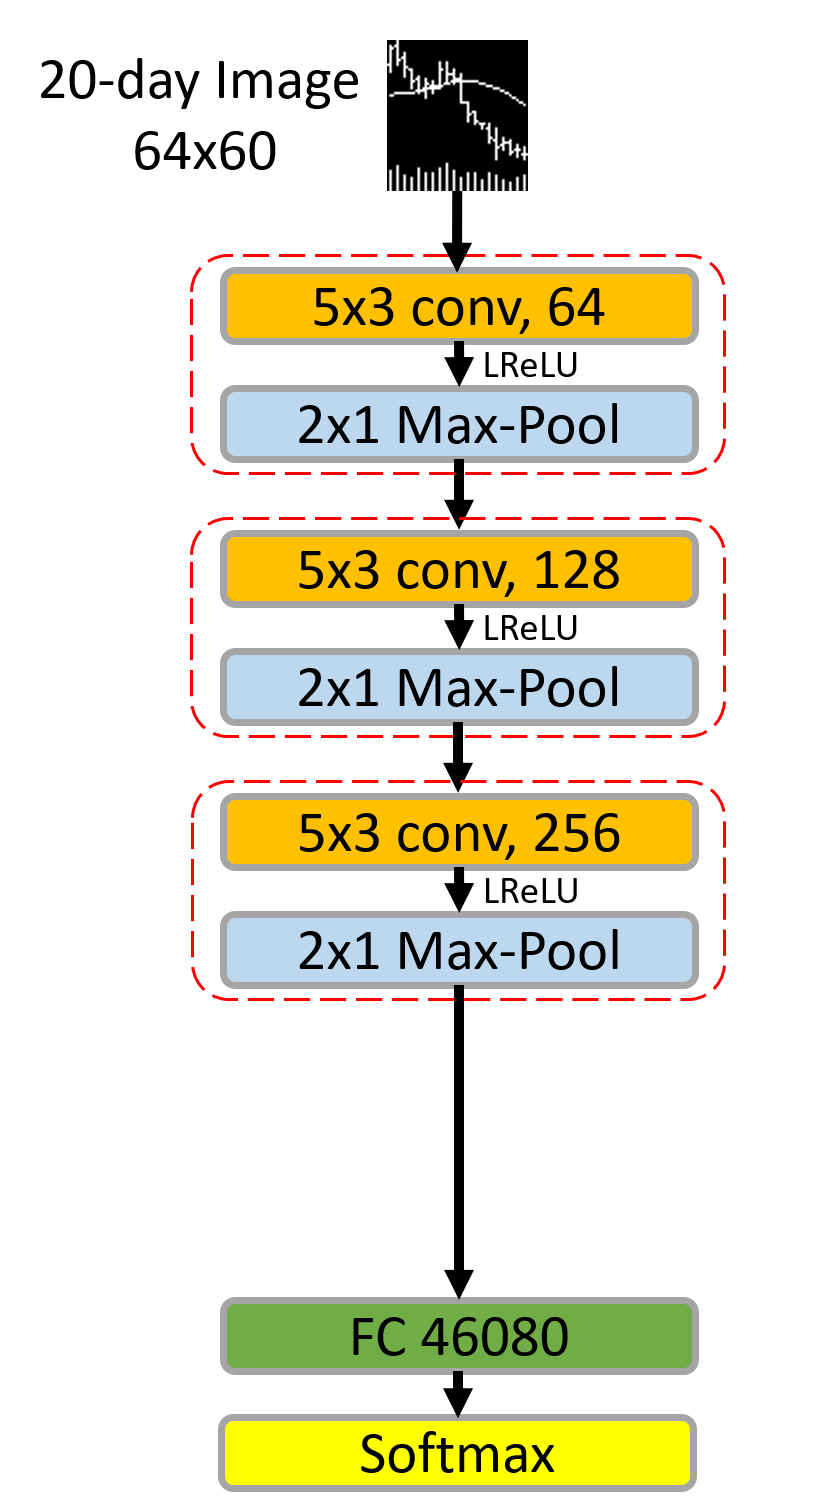
\includegraphics[width=0.6\linewidth]{3_1 Diagram of CNN Models.png}}
	\end{minipage}
	\hfill
	\begin{minipage}[c]{0.49\linewidth}
		\centering
		\adjustbox{valign=c}{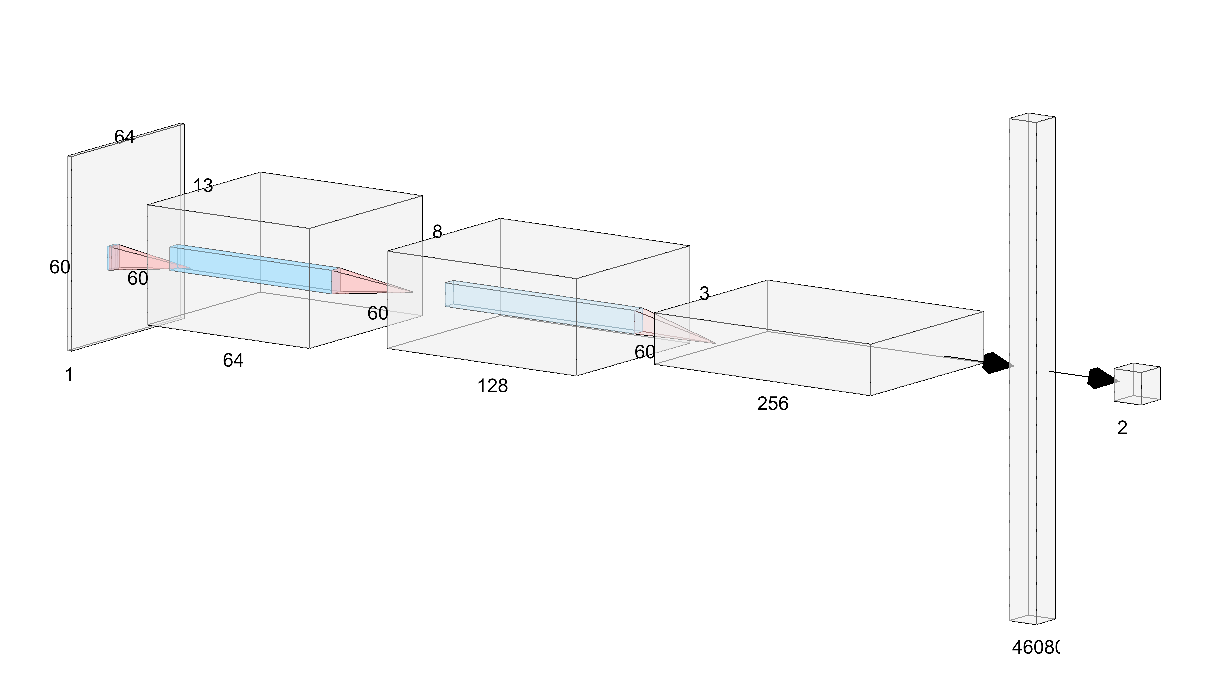
\includegraphics[width=0.8\linewidth]{3_2 Diagram of CNN Models.png}}
	\end{minipage}
	\caption{Examples of Final Image}
\end{figure}


\section{Working Flow}

\subsection{Data split}
Our workflow follows a standard procedure, starting with training the model, followed by model tuning, and finally making predictions. We divide the data samples into three sets: training, validation, and testing. Following the original paper, we also used a seven-year sample from 1993 to 2000 for training and validation. Within this sample, 70\% of the data was randomly selected for training the model, while the remaining 30\% was used for validation. The remaining twenty years of data were reserved as an out-of-sample test dataset.

\subsection{Regularization procedures}
To build a baseline CNN model for 20-day images, we incorporated several regularization techniques to combat overfitting and improve computational efficiency. We employed the Xavier initializer[2] to initialize the weights and enhance training efficiency and performance. Batch normalization[3] was integrated to address covariate shift and mitigate overfitting, stabilizing the network against input variations and facilitating faster convergence. Dropout regularization was applied to enhance model stability and reduce overfitting risks. Additionally, we used early stopping[4] to prevent overfitting by monitoring the model's performance on a validation set, stopping training when there was no improvement for two consecutive epochs, thus improving the model's generalization ability.

\subsection{Loss and evaluation}
\paragraph{$\bullet$ \emph {Cross Entropy Loss}}
In our prediction analysis, we treat it as a classification problem. The label for an image is defined as y = 1 for a positive subsequent return and y = 0 for a negative subsequent return.

By employing Cross Entropy Loss, we optimize our model's parameters to minimize the disparity between predicted probabilities and true labels. This enables the model to learn and improve its classification performance, ultimately enhancing its accuracy in predicting subsequent returns.

\begin{itemize}
    \setlength\itemindent{2em}
    \item[] \emph{$L_{CE}(y, \hat{y}) = -y\log(\hat{y}) - (1-y)\log(1-\hat{y})$}
\end{itemize}
	

We optimize the loss function using stochastic gradient descent (SGD) with the Adam algorithm. The initial learning rate is set to $1\times10^{-5}$, and we use a batch size of 128 to handle memory constraints. The training process involves 100 epochs, and we employ early stopping if the loss function does not improve on the validation set for two consecutive epochs.

\begin{figure}[H]
	\centering
	\begin{subfigure}[c]{0.49\linewidth}
		\centering	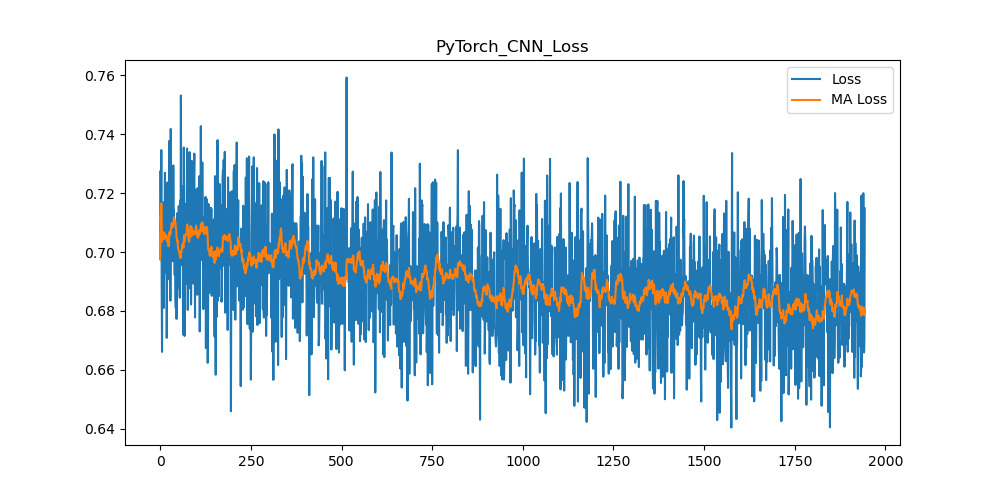
\includegraphics[width=0.8\linewidth]{4 CNN_classification_loss.png}
		\caption*{CNN classification loss}
	\end{subfigure}
	\hfill
	\begin{subfigure}[c]{0.49\linewidth}
		\centering
  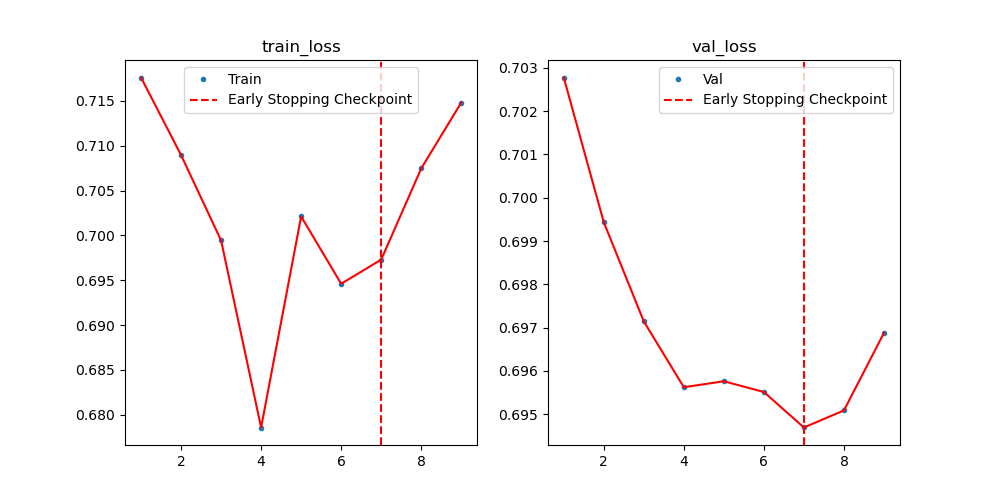
\includegraphics[width=0.8\linewidth]{5 CNN classification training and evaluation loss.png}
		\caption*{CNN classification training and evaluation loss}
	\end{subfigure}
	\caption{CNN classification training and evaluation loss}
\end{figure}

The loss function decreasing over time signifies the learning and enhancement of our model's classification performance. The plot includes a moving average of the loss function, which offers a smoother representation and highlights the overall trend. This moving average is computed by averaging the loss function values over a sliding window of 20 training iterations. Figure 5 presents a visual depiction of the training and evaluation loss functions for our CNN classification model. The x-axis denotes the number of training epochs, while the y-axis represents the value of the loss function.

In the training process, the left subplot shows the decreasing training loss function, indicating improved classification performance on the training data. The vertical red line represents the checkpoint where early stopping was applied to prevent overfitting.

The right subplot displays the evaluation loss function on the validation dataset. A decreasing trend in this loss function reflects the model's enhanced generalization ability on new data. The vertical red line corresponds to the early stopping checkpoint, demonstrating the model's strong generalization capabilities.

\paragraph{$\bullet$ \emph {Accuracy}}
The Accuracy metric is used to measure classification performance. It represents the ratio of correct predictions to the total number of predictions.

To calculate accuracy, we consider true positives (TP) and true negatives (TN). TP occurs when the predicted probability is greater than 50\% and matches a positive realized return. TN occurs when the predicted probability is less than 50\% and corresponds to a negative return. False positives (FP) and false negatives (FN) are incorrect predictions. FP indicates a positive prediction that doesn't align with a negative realized return, while FN indicates a negative prediction that doesn't match a positive realized return.

Accuracy is computed by summing the number of TP and TN predictions and dividing it by the total number of predictions, including TP, TN, FP, and FN. This formula provides a measure of the model's classification performance.

\begin{itemize}
    \setlength\itemindent{2em}
    \item[] \emph{$Accuracy = \frac{TP + TN}{TP + TN + FP + FN}$}
\end{itemize}

\paragraph{$\bullet$ \emph {Classification Performance}}
Table below illustrates the classification performances of our model after employing various regularization techniques. These procedures contribute to the improved classification performance of our model. 

\begin{table}[H]
  \centering
  \caption{Performance Comparison}
  \begin{tabular}{ccccc}
    \toprule
    & \multicolumn{2}{c}{Baseline (Paper)} & \multicolumn{2}{c}{Baseline (Replication)} \\
    \cmidrule(lr){2-3} \cmidrule(lr){4-5}
    & Test & Val & Test & Val \\
    \midrule
    Loss & 0.690 & 0.687 & 0.699 & 0.696 \\
    Accuracy & 0.533 & 0.542 & 0.522 & 0.529 \\
    \bottomrule
  \end{tabular}
\end{table}


The analysis reveals that the classification model demonstrates convergence as the number of iterations increases. The relationship between cross-entropy loss and accuracy over epochs indicates stable performance on the train and validation datasets, with a loss value of approximately 0.7 and an accuracy range of 0.50-0.54. The model's performance on the test dataset closely matches the results reported in the paper, with a loss value of 0.714 and an accuracy of 0.513. Overall, the model exhibits satisfactory convergence and generalization abilities.


\section{Extension}

\subsection{Ablation Studies}
To test the robustness of the CNN model, we follow the methodology outlined in Appendix B of the original paper and conduct a similar sensitivity analysis. We introduce various modifications to both the model architecture(e.g. number of convolution layers) and estimation(e.g. dropout rate or batch normalization schemes). The performance of the models are evaluated by loss, accuracy from test and validation process and the Pearsonr and Spearmanr correlation. Detailed variations of the model and their performance are shown in the table below.

\begin{table}[H] % 使用H选项禁止表格浮动
\centering
\caption{Sensitivity to Model Structure and Estimation, I20R20}
\begin{tabular}{ccccccccc} % 设置表格列数和对齐方式
\toprule % 第一条线
& \multicolumn{1}{c}{ Structure } & \multicolumn{2}{c}{Loss} & \multicolumn{2}{c}{Acc.} & \multicolumn{2}{c}{Correlation} \\
 \cmidrule(lr){3-4} \cmidrule(lr){5-6} \cmidrule(lr){7-8}
& & Test & Val & Test & Val & Spearman & Pearson \\
\midrule % 第二条线
$Baseline$ & $  $ & $0.699$ & $0.696$ & $0.522$ & $0.529$ & $0.035$ & $0.035$ \\
$Xavier$ & $ no $ & $0.701$ & $0.694$ & $0.520$ & $0.535$ & $0.036$ & $0.036$ \\
$Dropout$ & $ 0.75 $ & $0.700$ & $0.696$ & $0.522$ & $0.531$ & $0.035$ & $0.035$ \\
$ $ & $ 0.25 $ & $0.698$ & $0.692$ & $0.521$ & $0.535$ & $0.039$ & $0.039$ \\

$ Activation $ & $ LReLU $ & $0.700$ & $0.695$ & $0.519$ & $0.532$ & $0.034$ & $0.034$ \\
$ MaxPool Size $ & $ (2,2) $ & $0.700$ & $0.697$ & $0.520$ & $0.527$ & $0.037$ & $0.037$ \\
$ dilation/stride $ & $ (2,1)/(1,1) $ & $0.734$ & $0.734$ & $0.527$ & $0.525$ & $0.034$ & $0.034$ \\
$  $ & $ (1,1)/(3,1) $ & $0.700$ & $0.695$ & $0.520$ & $0.530$ & $0.034$ & $0.034$ \\
$  $ & $ (1,1)/(1,1) $ & $0.726$ & $0.718$ & $0.523$ & $0.532$ & $0.035$ & $0.035$ \\
$ Filters $ & $ 32 $ & $0.700$ & $0.695$ & $0.522$ & $0.532$ & $0.036$ & $0.036$ \\
$  $ & $ 128 $ & $0.700$ & $0.695$ & $0.520$ & $0.532$ & $0.035$ & $0.035$ \\

\bottomrule % 第三条线
\end{tabular}
\end{table}


The ablation studies reveal that CNN model’s performance is considerably robust and exhibits low sensitivity to alterations in modeling choices. 

\subsection{Interpretability}
CNN models are highly flexible and capable of automatically learning complex predictive patterns from data, eliminating the need for manual feature engineering. In this project, interpreting the model's decisions and understanding its reasoning process are crucial for gaining insights into the factors that influence stock price movements. 

We randomly select 10 images each for predicted movements “up” and “down” and the heap maps generated are shown below.

\begin{figure*}[!ht]
	\centering
 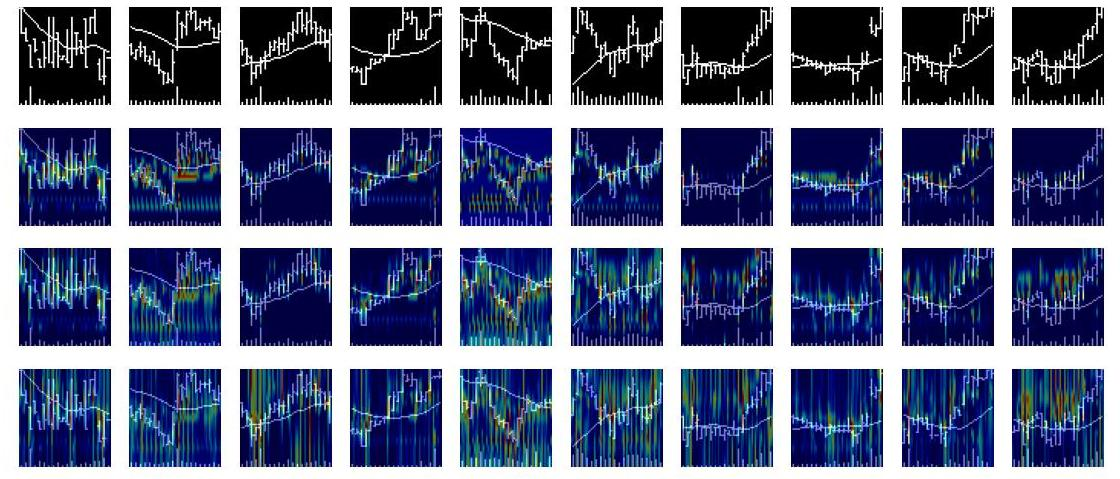
\includegraphics[width=0.6\textwidth]{8_1Images Receiving “Up” Signal(classification).jpg}
	\caption{Images Receiving “Up” Signal}
\end{figure*}

\begin{figure*}[!ht]
	\centering
	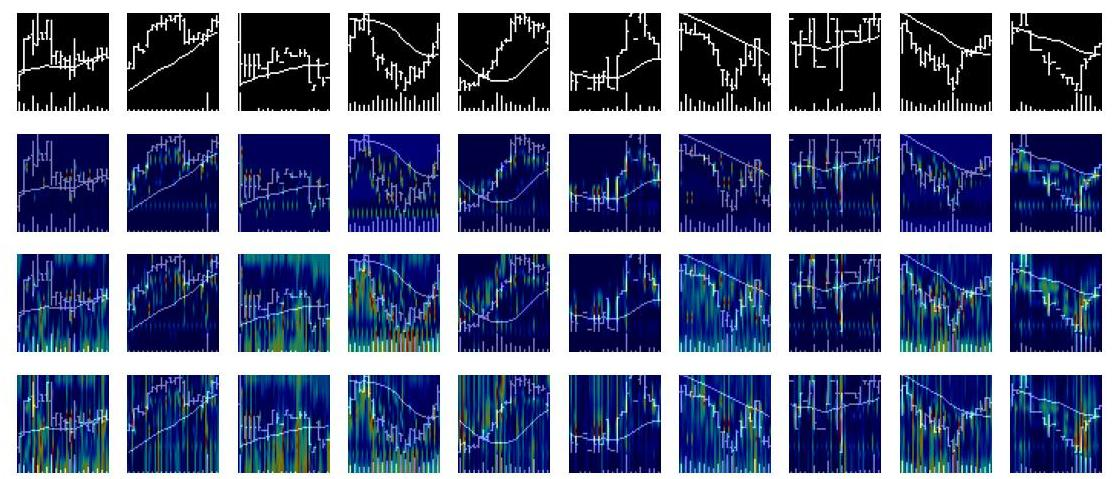
\includegraphics[width=0.6\textwidth]{8_2Images Receiving “Down” Signal(classification).jpg}
	\caption{Images Receiving “Down” Signal}
\end{figure*}

\subsection{Regression}
We expand our scope beyond binary classification and attempt to predict numerical values. The input remains to be the 20-day horizon images, representing historical stock movements and predictions are modified to be the next 5-day and 20-day holding period returns. To accommodate numerical predictions, we retain the overall structure of the CNN model while making two key changes: adjusting the loss function to Mean Squared Error (MSE) and changing the activation function in the output layer to linear instead of softmax. The figures below depict the MSE and early stopping checkpoint for both models.


\begin{figure}[H]
	\centering
	\begin{subfigure}[c]{0.49\linewidth}
		\centering
		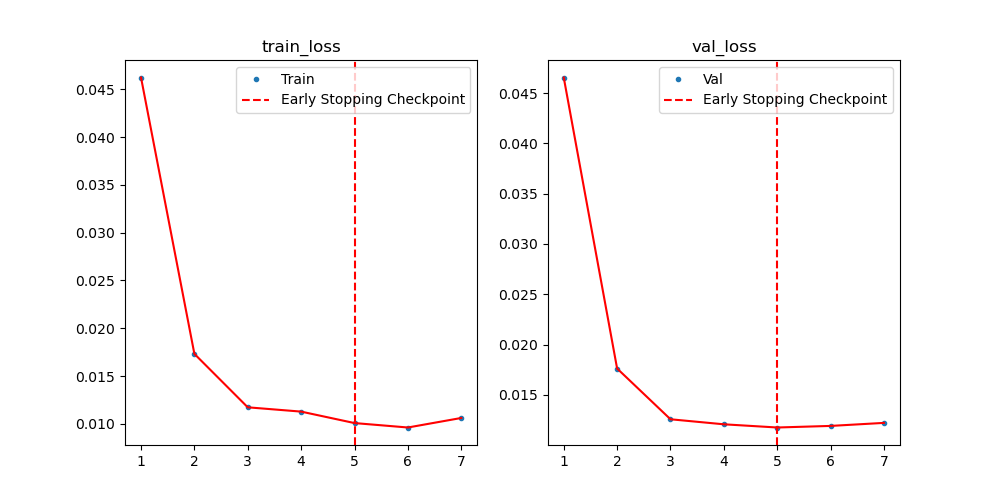
\includegraphics[width=0.8\linewidth]{9_3 CNN regression(ret_5) training and evaluation loss.png}
		\caption*{Regression(ret\_5) training and evaluation loss}
	\end{subfigure}
	\hfill
	\begin{subfigure}[c]{0.49\linewidth}
		\centering
		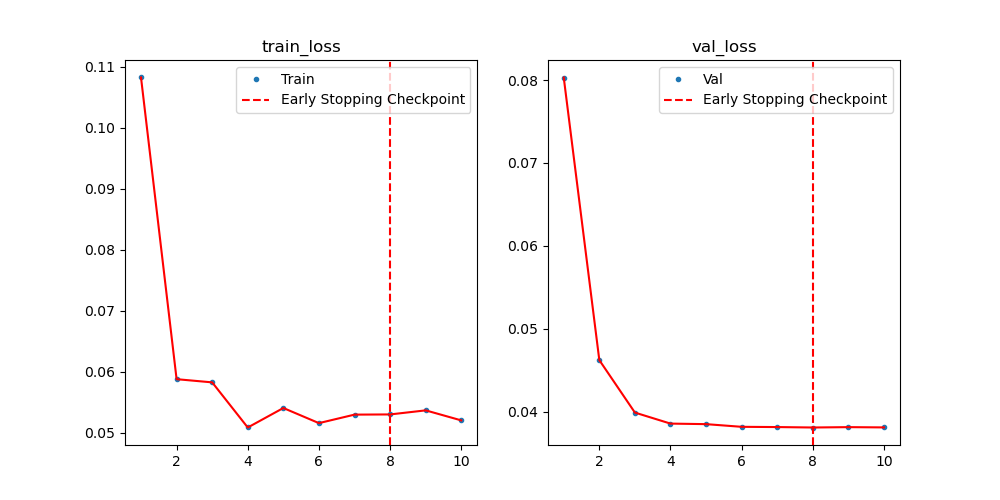
\includegraphics[width=0.8\linewidth]{10_3 CNN regression(ret_20) training and evaluation loss.png}
		\caption*{Regression(ret\_20) training and evaluation loss}
	\end{subfigure}
	\caption{CNN classification training and evaluation loss comparison}
\end{figure}


\begin{table}[H] % 使用H选项禁止表格浮动
  \centering
  \caption{Regression Performance Comparison}
  \begin{tabular}{ccccc} % 设置表格列数和对齐方式
    \toprule % 第一条线
    & \multicolumn{2}{c}{Ret(20)} & \multicolumn{2}{c}{Ret(5)} \\
    \cmidrule(lr){2-3} \cmidrule(lr){4-5}
    & Test & Val & Test & Val \\
    \midrule % 第二条线
    $R^2$ & $-0.0014271$ & $-0.0023383$ & $-0.0003037$ & $-0.0037581$ \\
    Loss & $0.0282230$ & $0.0380809$ & $0.0092049$ & $0.0117683$ \\ 
    MSE & $0.0270532$ & $0.0375446$ & $0.0081335$ & $0.0111302$ \\
    \bottomrule % 第三条线
  \end{tabular}
\end{table}

The  performance of both regression models are unsatisfactory, and we receive negative $R^{2}$ values. This could be attributed to multiple factors. One possible reason is insufficient input data, which can limit the model's ability to learn meaningful patterns and relationships. Additionally, the pooling and downsampling operations of CNN model may result in a loss of fine-grained information that is important for precise numerical predictions in regression tasks.

\section{Conclusion}

In this project, we successfully replicate the research paper by closely adhering to the original work's guidelines for data preparation, model design, workflow, and performance evaluation and our replication yields similar results. Moreover, we conduct ablation studies to assess the model's robustness, utilize Grad-CAM to interpret the CNN and identify crucial patterns for prediction, and extend our exploration to regression analysis. 

\section*{References}

\medskip

\small


[1] Jiang J, Kelly B T, Xiu D. (Re-) Imag (in) ing price trends[J]. Chicago Booth Research Paper, 2020 (21-01).

[2] Glorot, Xavier, and Yoshua Bengio, 2010, Understanding the difficulty of training deep feedforward neural networks, in Proceedings of the thirteenth international conference on artificial intelligence and statistics, 249–256.

[3] Ioffe, Sergey, and Christian Szegedy, 2015, Batch normalization: Accelerating deep network training by reducing internal covariate shift, arXiv preprint arXiv:1502.03167. 

[4]Srivastava, Nitish, Geoffrey Hinton, Alex Krizhevsky, Ilya Sutskever, and Ruslan Salakhutdinov, 2014, Dropout: A Simple Way to Prevent Neural Networks from Overfitting, The Journal of Machine Learning Research 15, 1929–1958.

[5] Z.C.Lipton.The Mythos of Model Interpretability.ArXive-prints, June 2016.

[6] Selvaraju, R. R., Cogswell, M., Das, A., Vedantam, R., Parikh, D., \& Batra, D. (2017). Grad-CAM: Visual Explanations from Deep Networks via Gradient-based Localization. In Proceedings of the IEEE International Conference on Computer Vision (ICCV), 618–626.


\section*{Group contribution}
Wang Jinyuan: Coding

Fu Yang: Coding Support and Report writing part of data, Architecture Design and Working Flow, Latex formatting

Luo Yuqing: Coding Support and Report writing part of Abstract, Introduction and Extension

Wang Tong: Coding Support

All members participate actively and equally contribute to this project.

\section*{Github link}
https://github.com/dboywjy/Re-Imaging-Price-Trends/tree/master

\end{document}


